% -*- TeX-engine: luatex -*-
\documentclass[presentation,aspectratio=43,10pt]{beamer}
\usepackage{template}
\renewcommand{\authorname}{Lawrence Mitchell\inst{*}}
\renewcommand{\authoremail}{\inst{*}\texttt{lawrence.mitchell@durham.ac.uk}}

\renewcommand{\sessionnumber}{1}
\renewcommand{\sessiontitle}{Introduction \& Overview}
\date{}

\begin{document}
\begin{frame}
  \maketitle
\end{frame}

\section{Introduction}

\begin{frame}
  \frametitle{What is the course about?}

  Saw (in Core I: High Performance Computing) different parallel
  programming paradigms.

  Parallelism helps to improve performance (runtime) of a code.

  \begin{challenge}{Question}
    Given some code, which I would like to make faster, how do I know
    \emph{what} to do?
  \end{challenge}
  \pause
  \begin{answer}{Performance models \& measurements}
    We can treat the computer as an experimental system

    $\Rightarrow$ perform measurements of the performance

    $\Rightarrow$ construct \emph{models} that explain performance

    $\Rightarrow$ apply appropriate optimisations
  \end{answer}
\end{frame}

\begin{frame}
  \frametitle{Course overview (not in order, approximate)}
  \begin{itemize}
  \item Computer architecture overview
  \item Fundamentals of performance engineering
  \item Tools: CPU topology and \emph{affinity}
  \item Roofline performance model
  \item Tools: Performance counters
  \item Vectorisation (SIMD programming)
  \item Data layout transformations
  \end{itemize}
\end{frame}

\begin{frame}
  \frametitle{What you need}
  \begin{itemize}
  \item The toolchain we'll use is available on Linux machines (but
    not Windows/Mac)
  \item I recommend using Hamilton (you should already have accounts
    from Core I)
  \item[$\Rightarrow$] Short howto from Core I website. Exercises will
    also recap some of this material.
  \end{itemize}
\end{frame}

\section{Resources in stored program computers}

\begin{frame}
  \frametitle{Hardware for programmers}
  \begin{center}
    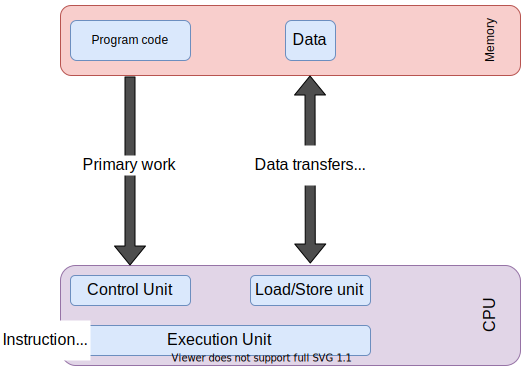
\includegraphics[height=0.8\textheight]{figures/CPU}
  \end{center}
\end{frame}

\begin{frame}
  \frametitle{Resource bottlenecks: instructions}
  \begin{block}{Instruction execution}
    How fast the CPU retires instructions.

    Primary resource of the processor. Primary hardware design goal is to
    \emph{increase} instruction throughput (instructions/second).
  \end{block}
  \begin{challenge}{Mismatch}
    Instructions are ``work'' as seen by processor designers.

    Not all instructions are considered ``work'' by software
    developers (you!).
  \end{challenge}
\end{frame}
\begin{frame}[fragile]
  \frametitle{Resource bottlenecks: instructions}
  \begin{exampleblock}{Adding two arrays}
\begin{minted}{c}
               for (int i = 0; i < N; i++)
                 a[i] = a[i] + b[i];
\end{minted}
    \begin{columns}[t]
      \begin{column}{0.45\textwidth}
        User view

        Work is $N$ flops (additions)
      \end{column}
      \begin{column}{0.45\textwidth}
        Processor view

        Work is $6N$ instructions
\begin{minted}{c}
.top
LOAD r1 = a[i]
LOAD r2 = b[i]
ADD  r1 = r1 + r2
STORE a[i] = r1
INCREMENT i
GOTO .top IF i < N 
\end{minted}
      \end{column}
    \end{columns}
  \end{exampleblock}
\end{frame}

\begin{frame}[fragile]
  \frametitle{Resource bottlenecks: data transfer}
  \begin{block}{Data Transfer}
    Data movement (from memory to CPU and back) is a
    \emph{consequence} of instruction execution and considered a
    secondary resource. Maximum bandwidth (bytes/second) determined by
    rate at which load/store instructions can be executed and hardware limits.
  \end{block}
  \begin{exampleblock}{Data movement adding two arrays}
\begin{minted}{c}
for (int i = 0; i < N; i++)
  a[i] = a[i] + b[i];
\end{minted}

    Data transfers (double precision floats):
\begin{minted}{c}
LOAD  r1 = a[i] /* 8 bytes */
LOAD  r2 = b[i] /* 8 bytes */
STORE a[i] = r1 /* 8 bytes */
\end{minted}

    24 bytes of data movement per loop iteration.
  \end{exampleblock}
\end{frame}

\begin{frame}
  \frametitle{Core question}
  To understand the performance of some code we must answer

  \begin{challenge}{Question}
    \begin{center}
      {\Large What is the resource bottleneck? }
    \end{center}
    \begin{itemize}
    \item Data transfer?
    \item Instruction execution?
    \end{itemize}
  \end{challenge}
  \pause
  \begin{answer}{Answer}
    We will see how to answer these questions in this course through a
    combination of measurements and models.
  \end{answer}
\end{frame}

\begin{frame}
  \frametitle{Real hardware vs.~models}
  Model of hardware as presented by programming languages is von
  Neumann model.

  Sequential execution of instructions, each instruction completes
  before next one starts.

  \begin{center}
    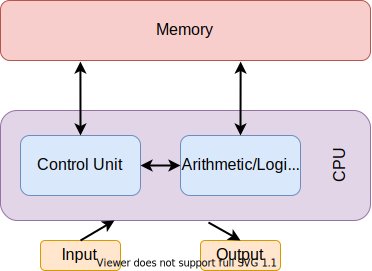
\includegraphics[height=0.6\textheight]{figures/vonneumann}
  \end{center}
\end{frame}

\begin{frame}[fragile]
  \frametitle{Problem}
  \begin{itemize}
  \item CPUs operate at a certain frequency, we will count time in
    terms of clock ``cycles''. For example, a 1GHz processor runs at one
    billion cycles per second.
  \item Due to the complexity of modern chips, most instructions have
    a \emph{latency} of \emph{more than one} clock cycle.
  \end{itemize}
  \begin{columns}
    \begin{column}{0.35\textwidth}
      \begin{exampleblock}{Example: addition loop}
\begin{minted}{c}
 LOAD r1 = a[i]
 LOAD r2 = b[i]
 ADD  r1 = r1 + r2
 STORE a[i] = r1
 INCREMENT i
\end{minted}
      \end{exampleblock}
    \end{column}
    \begin{column}{0.55\textwidth}
      Suppose that the CPU can execute one instruction per cycle. If
      every instruction has a latency of one cycle, then there are no
      ``wasted'' cycles.
      
      If \texttt{ADD} has latency of three cycles, then there are
      two wasted cycles (between the \texttt{ADD} and the
      \texttt{STORE}).
    \end{column}
  \end{columns}
\end{frame}
\begin{frame}
  \frametitle{A picture}
  \begin{center}
    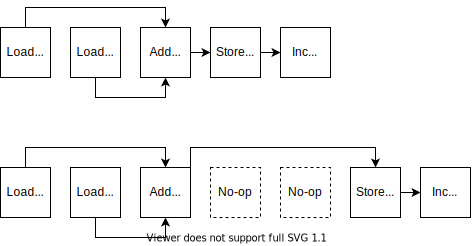
\includegraphics[width=\textwidth]{figures/addlatency}
  \end{center}
\end{frame}

\begin{frame}
  \frametitle{Strategies for faster chips}
  \begin{enumerate}
  \item Increase clock speed (more cycles per second)
  \item Parallelism (of various kinds)
  \item Specialisation (for example optimised hardware for computing divisions)
  \end{enumerate}
\end{frame}

\begin{frame}
  \frametitle{Increasing clock speed}
  \begin{center}
    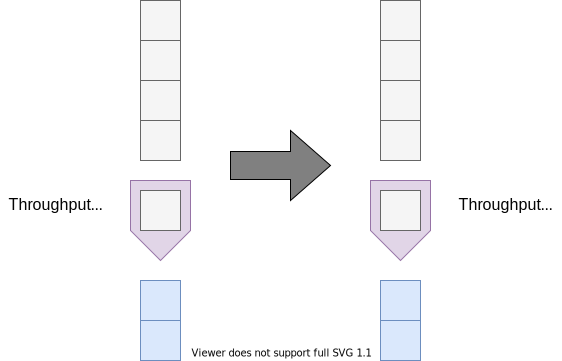
\includegraphics[height=0.45\textheight]{figures/clockincrease}
  \end{center}

  \begin{answer}{Easy for the programmer}
    Architecture is unchanged, everything just happens faster!
  \end{answer}
  \begin{challenge}{Limitations}
    Limited by physical limitations on cooling.

    Clock speeds have been approximately constant for 10 years.
  \end{challenge}
\end{frame}

\begin{frame}
  \frametitle{Increasing parallelism}
  \begin{center}
    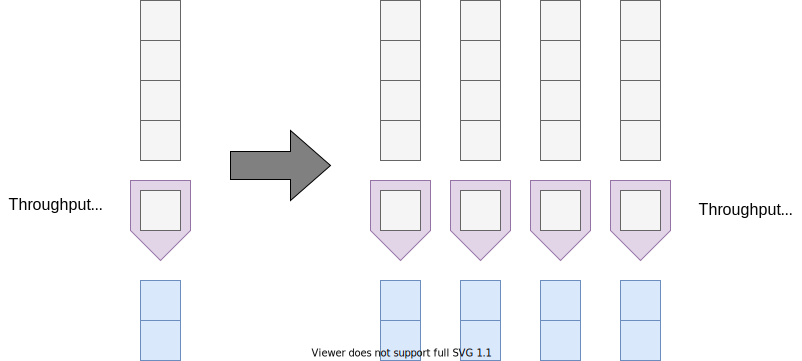
\includegraphics[height=0.5\textheight]{figures/parallelismincrease}
  \end{center}

  \begin{challenge}{Problems}
    Need enough parallel work

    No dependencies between work

    Mostly pushes problem onto programmer
  \end{challenge}
\end{frame}

\begin{frame}
  \frametitle{Instruction-level parallelism: pipelining}
  \begin{block}{Pipelining}
    Rather than performing instruction fetch, decode, execute, and
    writeback in one go, separate them into a pipeline.
  \end{block}
  \begin{center}
    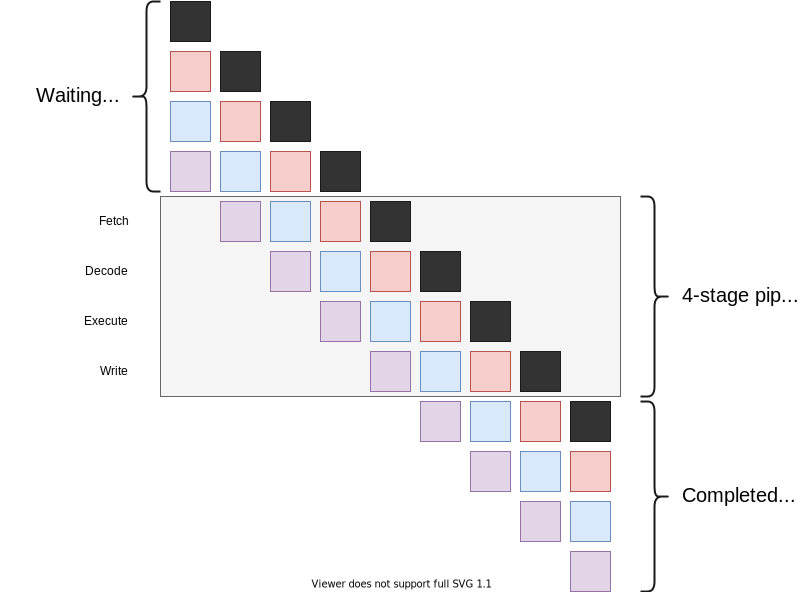
\includegraphics[height=0.7\textheight]{figures/pipeline}
  \end{center}
\end{frame}

\begin{frame}
  \frametitle{Instruction-level parallelism: superscalar}
  \begin{block}{Superscalar execution}
    Most modern chips can issue more than one instruction per cycle.

    Instructions with no dependencies can be issued simultaneously.
  \end{block}
  \begin{center}
    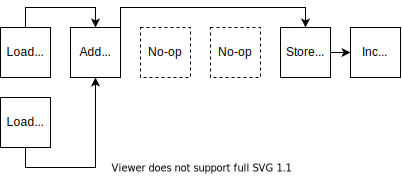
\includegraphics[width=0.9\textwidth]{figures/addsuperscalar}
  \end{center}
\end{frame}

\begin{frame}
  \frametitle{Instruction-level parallelism: out-of-order}
  \begin{block}{Out-of-order execution}
    Execute instructions in an ordering based on availability of \emph{input
      data} and \emph{execution units} rather than the order in the program.
    
    Keeps more of the execution units busy.
  \end{block}

  \begin{center}
    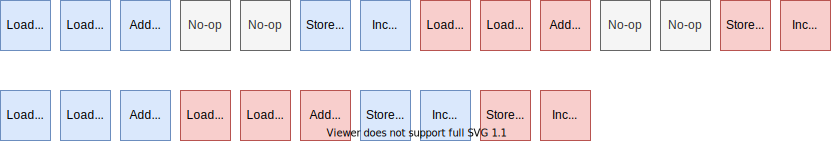
\includegraphics[width=0.9\textwidth]{figures/addoutoforder}
  \end{center}
\end{frame}

\begin{frame}[fragile]
  \frametitle{Data parallelism: SIMD vectorisation}
  \begin{block}{SIMD}
    We mostly consider ``single-core'' performance in this course. \emph{Vectorisation} is critical for single-core performance.
  \end{block}

  \begin{exampleblock}{Summing arrays again}
\begin{minted}{c}
double *a, *b, *c;
...
for (size_t i = 0; i < N; i++)
  c[i] = a[i] + b[i];
\end{minted}

    We've seen that instruction throughput can be a bottleneck here.

    One way chip designers have ``fixed'' this is to make individual
    instructions operate on more data at once $\Rightarrow$ vectorisation.
  \end{exampleblock}
\end{frame}

\begin{frame}[fragile]
  \frametitle{SIMD execution}
  \begin{columns}
    \begin{column}{0.4\textwidth}
\begin{minted}{c}
double *a, *b, *c;
...
for (i = 0; i < N; i++)
  c[i] = a[i] + b[i];
\end{minted}

      \vspace{\baselineskip}
      Register widths:
      \vspace{\baselineskip}
      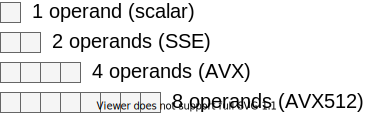
\includegraphics[width=\textwidth]{figures/registerwidth}
    \end{column}
    \begin{column}{0.6\textwidth}
      \only<1>{Scalar addition, 1 output element per instruction.
        \begin{center}
          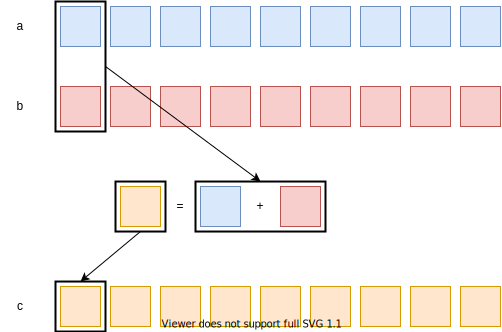
\includegraphics[width=0.9\textwidth]{figures/scalaradd}
        \end{center}}
      \only<2>{AVX addition, 4 output elements per instruction.
        \begin{center}
          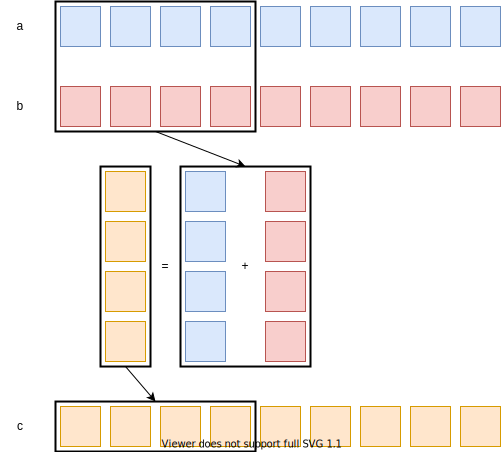
\includegraphics[width=0.9\textwidth]{figures/vectoradd}
        \end{center}}
    \end{column}
  \end{columns}
\end{frame}

\section{Example and exercise}

\begin{frame}[fragile]
  \frametitle{A ``simple'' example: sum reduction}
  \begin{columns}
    \begin{column}{0.4\textwidth}
\begin{minted}{c}
float c = 0;
for (i = 0; i < N; i++)
  c += a[i];
\end{minted}
    \end{column}
    \begin{column}{0.6\textwidth}
      Single precision sum of all values in a vector, on an
      AVX-capable core (vector width 8).

      How fast can this code run if all data are in L1 cache?
    \end{column}
  \end{columns}
  \begin{itemize}
  \item Loop-carried dependency on summation variable
  \item Execution stalls at every add until the previous one completes.
  \end{itemize}
\end{frame}

\begin{frame}[fragile]
  \frametitle{Applicable peak}
  \begin{columns}
    \begin{column}{0.4\textwidth}
      Scalar code

\begin{minted}{c}
float c = 0;
for (i = 0; i < N; i++)
  c += a[i];
\end{minted}

      Assembly pseudo-code
      
\begin{minted}[mathescape=true,escapeinside=||]{c}
LOAD r1.0 |$\gets$| 0
i |$\gets$| 0
loop:
  LOAD r2.0 |$\gets$| a[i]
  ADD  r1.0 |$\gets$| r1.0 + r2.0
  i |$\gets$| i + 1
  if i < N: loop
result |$\gets$| r1.0
\end{minted}

    \end{column}
    \begin{column}{0.5\textwidth}
      ADD has latency of 1 cycle (per Intel), but we're only using one
      of the eight SIMD lanes for each instruction.

      \begin{center}
        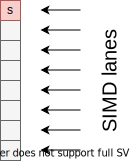
\includegraphics[height=0.5\textheight]{figures/scalarregisteruse}
      \end{center}

      Runs at 1/8 of possible ADD peak.
    \end{column}
  \end{columns}
\end{frame}

\begin{frame}[fragile]
  \frametitle{Applicable peak}
  \begin{columns}
    \begin{column}{0.6\textwidth}
      SIMD vectorisation

      Assembly pseudo-code
      
\begin{minted}[fontsize=\scriptsize, mathescape=true,escapeinside=||]{c}
LOAD [r1.0, ..., r1.7] |$\gets$| [0, ..., 0]
i |$\gets$| 0
loop:
  LOAD [r2.0, ..., r2.7] |$\gets$| [a[i], ..., a[i+7]]
  ADD  r1 |$\gets$| r1 + r2 // SIMD ADD
  i |$\gets$| i + 8
  if i < N: loop
result |$\gets$| r1.0 + r1.1 + ... + r1.7
\end{minted}

    \end{column}
    \begin{column}{0.3\textwidth}
      Using all eight SIMD lanes

      \begin{center}
        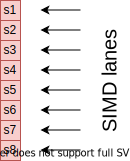
\includegraphics[height=0.5\textheight]{figures/vectorregisteruse}
      \end{center}

      Runs at ADD peak.
    \end{column}
  \end{columns}
\end{frame}

\begin{frame}
  \frametitle{Exercise: benchmarking sum reduction}

  \begin{itemize}
  \item Split into small groups, each group should have at least one
    person with a Hamilton account.
  \item Goal is to benchmark sum reduction to see if we observe this
    ``theoretical'' effect.
  \item $\Rightarrow$ over to you. Please ask questions!
  \end{itemize}
  \begin{center}
    Exercises, and notes, live at

    \url{https://teaching.wence.uk/comp52315/}
  \end{center}
\end{frame}

\begin{frame}
  \frametitle{Conclusions}
  \begin{itemize}
  \item Modern computer hardware is quite complex
  \item For simple things we can work out what the performance limits
    will be
  \item Typically must benchmark to confirm hypotheses
  \item Next, we'll look at the memory hierarchy and start
    constructing models of performance.
  \end{itemize}
\end{frame}

\end{document}
